%!TEX root = ./main.tex
\chapter{Implementation\label{Tasks}}

\section{IPv6 Support}
\subsection{IPv6 and the SWITCH Network}
Since the end of January 2011, there are no more Internet Protocol version 4 (IPv4) address blocks available at IANA\footnote{Internet Assigned Numbers Authority \url{http://www.iana.org}}. Hence, only the region Internet registries (RIR) are able to allocate few IPv4 address blocks. Estimations \cite{Huston:potaroo} predicts the first RIR IPv4 address pool exhaustion in mid 2011 (APNIC\footnote{Asia and Pacific Network Information Center \url{http://www.apnic.net}}). This means that there are no longer IPv4 address blocks available for the affected region. Hence, this may influence the growth of the Internet as a whole. The fact of IPv4 address depletion is known since decades and a working solution is provided by version 6 of the Internet Protocol (IPv6). However, the deployment of IPv6 is running very slowly, although, IPv6 was officially announced as successor of IPv4 in December 1998 by the RFC2460.

The Swiss national research and education network SWITCH\footnote{SWITCH: \url{http://www.switch.ch}} is providing by June 2004 a fully enabled dual-stack backbone network for the Swiss universities \cite{SWITCH:IPv6}. Seven years later, none of the Swiss universities have fully enabled IPv6 on their own networks. SWITCH states that "there are technologies that are exceedingly important but slow to get off the ground. IPv6, the new version of the Internet protocol, is one of these."\cite{SWITCH:IPv6_incent}. Therefore, SWITCH have recently launched an incentive program to motivate the universities to enable IPv6 on their network \cite{SWITCH:IPv6}. Hopefully, Swiss universities will deploy IPv6 on their networks in the near future to be ready for the future of the Internet.

Since FACT mainly intents to analyze the traffic from the SWITCH network and other network operators, the FACT code framework has to be able to process IPv6 flow-level traces. This adaption to fully support IPv6 is done as an essential part of this semester thesis. In section \ref{RES_IPV6}, some results about the traffic volumes within the SWITCH network are presented.

\subsection{IPv6 and FACT}
Since FACT processed so far only IPv4 flows - all IPv6 flows were filtered and dropped - there are several adjustments to be made in the framework of FACT. One aim of this semester thesis is to enable IPv6 in FACT such that FACT is able to track connectivity issues for IPv4 and IPv6 networks.

The work for enabling IPv6 in FACT contained the following parts:

\begin{itemize}
	\item Creation of a filter for all IPv4 connections (FilterIPv4), so that only IPv6 connections can be processed, e.g. for IPv6
	 only networks, analogous to FilterIPv6.
	\item Adjustment of the filter for incoming/outgoing connections(FilterInOut), in particular the configuration file for the FilterINOUT. This configuration file contains all prefixes of the home network - in this case all prefixes of the SWITCH network. For creating this file automatically, a little perl script (switchextract.pl) is included in the tool folder of the FACT code. This script needs the output of bgpdump for the desired timeframe. Moreover, this script is generating a file prefixes.txt, which is needed by the analyser of FACT.
	\item Adjustment of all prefix routines for aggregating and matching IPv6. Since the analyser of FACT aggregates IPv4 hosts up to a /24 network, IPv6 hosts are aggregated up to a /48 network by the analyser.
	\item Separation of IPv4 and IPv6 flows into own connection matrices - one for matching IPv4 flows and the other for IPv6 flows.
	\item Adoption of the analyser to analyze each connection matrix and to output the analyser results into an own IPv4 and IPv6 folder.
\end{itemize}

\subsubsection{Problems}

While enabling IPv6 in FACT, several problems appeared. Since this task was the first to implement, a deep contemplation and comprehension of the existing FACT code framework was inevitable, which was very time consuming and required several further assistance by the developer of FACT. Afterwards, the essential parts of enabling IPv6 had to be identified. The key troubles have been appeared while implementing the separation of flows into two separate connection matrices. The working solution is to initialize for each type of flow - IPv4 and IPv6 - an own connection matrix hash table (Connection\_Matrix\_HT). After solving this issue, the residual tasks of enabling IPv6 in FACT were quite straightforward.

\section{NfDump}

\subsection{NfDump in a nutshell}
NfDump is a toolset similar to tcpdump, but for collecting and processing flow level traces instead of packet level traces. It is developed by SWITCH and widely used by network operators over the world. NfDump supports netflow versions 5, 7 and 9 \cite{nfdump:SF}.

The NfDump toolbox mainly consists of the following parts:
\begin{description}
	\item[nfcapd] is the \emph{netflow capture deamon}. nfcapd is able to collect netflow data from several exporting routers and saves the collected data.
	\item[nfdump] is the main processing tool. It allows the user for example to sort the data and to create some top-N-statistics.
	\item[nfprofile] is the filter instance of nfdump. Nfprofile is able to filter the stored data according to a predefined set of filter rules and saves the filtered data.
	\item[nfreplay]	is intended to replay the saved flows. This means that nfreplay is able to send the stored data to another host in the network.
\end{description}
\begin{figure}[ht!]
	\centering
	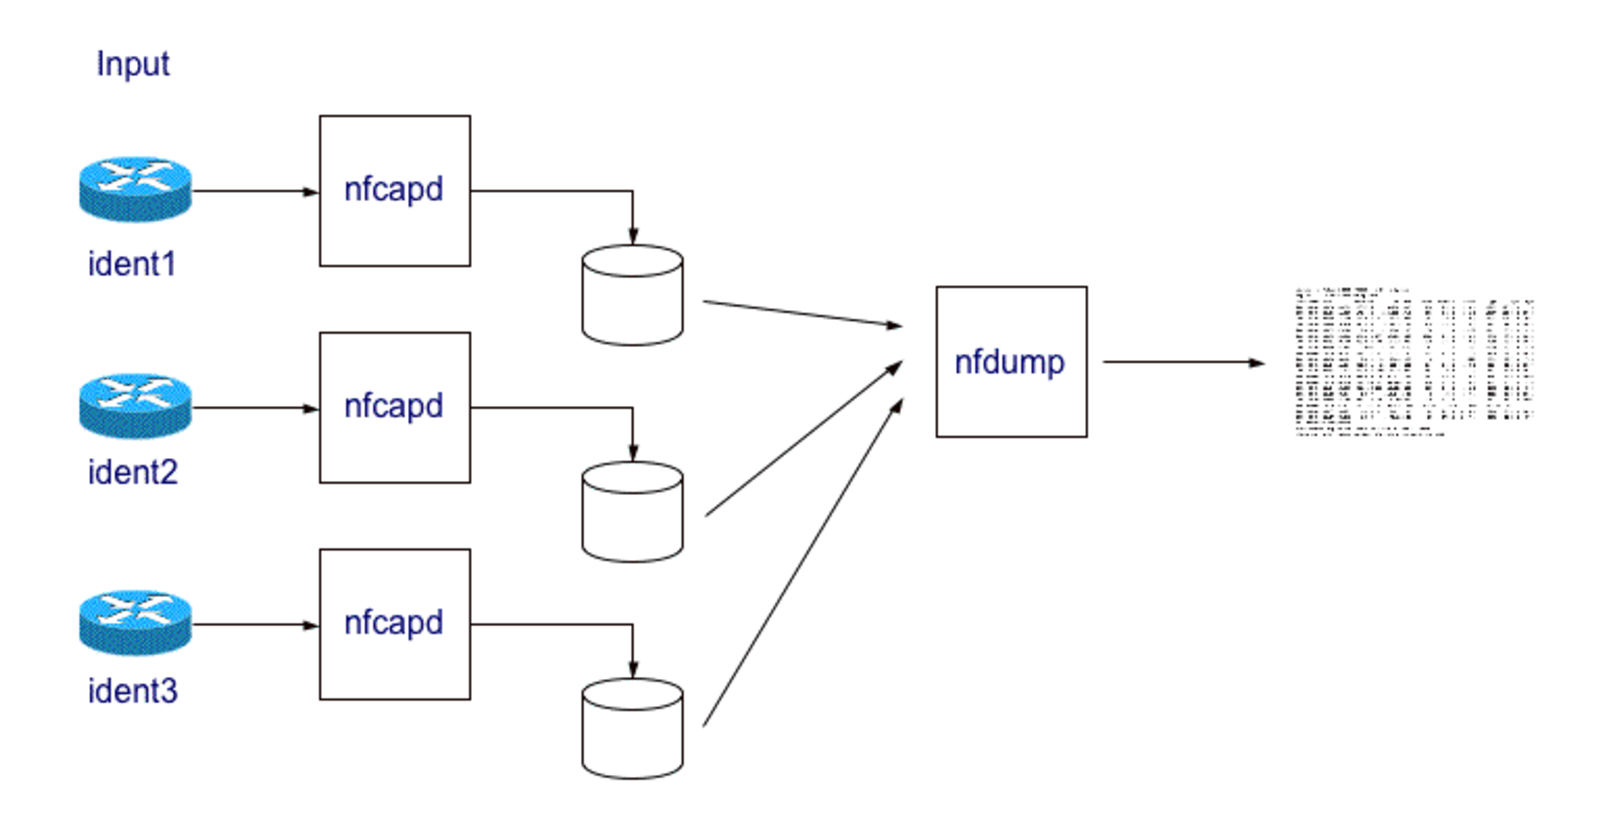
\includegraphics[width=160mm]{images/nfdump}
	\caption{functional overview of NfDump \cite{nfdump:SF}}
	\label{fig:nfdump}
\end{figure}
The entire toolbox is called NfDump, while the main processing tool is called nfdump.
Figure \ref{fig:nfdump} shows systematically how nfcapd and nfdump are interacting. Nfcapd is collecting netflow exports from routers and saving them into predefined directories. Then nfdump is able to get these saved traces and is processing these traces into some statistics.


\subsection{Integration with NfDump}
The main motivation of integrate NfDump data is that FACT has to be able to read some standardized data format. Up to now, FACT is only processing a proprietary netflow format of the Communication Systems Group (CSG). A big goal of FACT is that it will be deployed at SWITCH or other network operators in the near future. Hence, the data input format must be somehow standardized to guarantee the interoperability with the flow-level traces of the network operator which are often already captured with nfcapd. For example SWITCH is capturing netflow traces with nfcapd. Therefore, this task was about to integrate the ability of reading nfdump data as input data in FACT.

The jobs related to the integration with NfDump were the following:
\begin{itemize}
	\item Adjustment of the main routine connectivity\_extract, so that it accepts a nfdump input data folder as argument.
	\item Adoption of the data parser which calls nfdump to extract the needed information out of the data files and correctly initializes the connection entries.
\end{itemize}

Because of the limited amount of time, only an input of comma separated value (csv) output of nfdump is implemented so far. An direct import of the binary nfdump data format is planned and will be finished soon.

\subsubsection{Problems}
Because NfDump is a open-source software, the source code is publicly available and thus an insight into this code yields the functionality of NfDump including its data format. There is also an example for a nfdump data reader included in the sources. Although, due to the lack of time, only a csv data input was implemented. This is done through calling the nfdump function directly from the ruby C++ extension of the data parser and then parsing the piped output. The function call includes a special format and is specified as the following:

\begin{lstlisting}[caption=nfdump function call with special format specification for FACT csv input, language=sh]
	nfdump -m -o "fmt:%ts,%te,%sa,%sp,%da,%dp,%pr,%ra,%nh,%in,%out,%pkt,%byt" -r nfcapd_dir
\end{lstlisting}

After exporting some local traces with fprobe\footnote{fProbe \url{http://fprobe.sourceforge.net}} and capturing these traces with nfcapd, some tests have been made. During these tests, a weird bug in the nfdump code\footnote{NfDump version 1.6.2} have been discovered. This bug disposed nfdump to setting some fields in a random manner, e.g. the router address (\%ra). After confirming this bug on several systems, Peter Haag from SWITCH was contacted and notified about this bug. The root cause of this bug was a falsely initialized master record of an flow within the nfdump data. For fixing this bug a patch was provided and since February 2011 the new version 1.6.3 of nfdump is available with included patch.


\section{Smart Reporting Engine}

\subsection{Approach}
The main goal of this smart reporting engine is to provide an easily understandable overview of the connectivity situation for a given period. Since the analyser is creating information in several distributed files, the reporter must collect, combine and process this information. One important part of the reporting engine is the classification of the connectivity problem. An important role in classifying the connectivity problems is the \emph{severity}, which means how many internal hosts are affected by a problem. A problem is more severe the more internal hosts are affected. For classifying connectivity issues thresholds are playing an important role as well. The border between a classification of a non-severe problem and a severe problem is called threshold. This threshold must be set cleverly in order to achieve a good classification. The intention of the smart reporting engine was to keep the model as simple as possible, regardless to achieve an usable classification with a low false positive rate. This is done with the so called \emph{8to8 model}.

\subsubsection{8to8 Model}
The basic idea of this 8to8 model is that if there are a large amount of network users during the day (from 8am till 8pm), a lot of minor connectivity problems may be detected. Therefore, to classify only the really important connectivity issues a higher threshold value must be set than the threshold of the night. So according to the time of the report, a threshold variable is set to threshold\_day or threshold\_night.

To classify a connectivity issue several variables are required and defined as follows:
\begin{description}
	\item[\texttt{score}] is a count variable. Upon this variable the decision is made.
	\item[\texttt{top\_number}] is the number of prefixes in the top five problem causing prefixes and can be an element of $\{0,1,2,3,4,5\}$
	\item[\texttt{top\_sum}] is the sum of the severity from each prefix of top five problem causing prefixes.
	\item[\texttt{problem\_sum}] is the overall sum of the severity from each problem causing prefix, i.e. not only from the top five prefixes.
\end{description}
In order to capture several events this count variable is set by the following three events:
\begin{enumerate}
	\item \texttt{top\_sum} exceeds the threshold which means that there are enough internal hosts affected to form a severe connectivity problem.
	\item \texttt{problem\_sum} exceeds the \texttt{top\_sum} by factor 2: This means that there are a lot of minor problems so that more than twice as many users are affected by these minor issues than by the five major issues.
	\item \texttt{top\_number}: The number of prefixes in the top five - usually less than 5 - is intended to capture severe routing failures.
\end{enumerate}

\begin{table}[ht!]
	\begin{center}
		\begin{tabular}{|l|p{12cm}|}
			\hline
			\textbf{Classification} & \textbf{Explanation}\\
			\hline\hline
			unlikely & \texttt{top\_sum} does not exceed the threshold and the overall \texttt{problem\_sum} is not twice the \texttt{top\_sum}. This means that there are not many connectivity issues and therefore, probability of a severe connectivity issue is unlikely.\cr
			\hline
			very likely & \texttt{top\_sum} exceeds the threshold and either there are five top five failed prefixes or there are a lot of minor problems, i.e. \texttt{problem\_sum} exceeds twice the \texttt{top\_sum}. \cr
			\hline
			likely & everything else, individual resolution and classification is required. \\
			\hline
		\end{tabular}

		\caption{Classifications}
		\label{tab:classification}
	\end{center}
\end{table}

\subsection{Report}
The implemented reporting engine is creating three sections in a report file:
\begin{itemize}
	\item \texttt{Connectivity Problem}: Classification of the likelihood of a connectivity issue during the reporting period. Table \ref{tab:classification} shows the different classifications and their explanations.
	\item \texttt{Top Problems}: sorted delineation of the five most severe prefix outages.
	\item \texttt{Problem Structure}: well-arranged overview of each prefix outage in a tree display. The top five problem causing prefixes are partitioned into the top five problem causing /24 network of this prefix and these are again partitioned into the top five problem causing hosts in this network.
\end{itemize}
\begin{table}[t]
	\newpage
	\begin{lstlisting}[caption=an excerpt of a report showing the presentation of the problem in tree structure]
FACT REPORT
-----------

EPOCH: 1283159700
DATE: 2010-08-30 11:15:00 +0200
:::::::::::::::::::::::::::::::::::::::
CONNECTIVITY PROBLEM: VERY LIKELY
:::::::::::::::::::::::::::::::::::::::

TOP PROBLEMS:
1: PREFIX: 88.221.XXX.0/21, SEVERITY: 615
2: PREFIX: 92.123.XXX.0/22, SEVERITY: 547
3: PREFIX: 92.122.XXX.0/22, SEVERITY: 204
4: PREFIX: 95.101.XXX.0/22, SEVERITY: 200
5: PREFIX: 207.107.XXX.0/16, SEVERITY: 2


PROBLEM STRUCTURE:
1: PREFIX: 88.221.XXX.0/21, SEVERITY: 615
    1.1 NET: 88.221.XXX.0/24, SEVERITY: 154
       |- HOST: 88.221.XXX.XXX/32, SEVERITY: 1
       |- HOST: 88.221.XXX.XXX/32, SEVERITY: 1
       |- HOST: 88.221.XXX.XXX/32, SEVERITY: 1
       |- HOST: 88.221.XXX.XXX/32, SEVERITY: 1
       |- HOST: 88.221.XXX.XXX/32, SEVERITY: 1
    1.2 NET: 88.221.XXY.0/24, SEVERITY: 142
       |- HOST: 88.221.XXY.XXX/32, SEVERITY: 1
       |- HOST: 88.221.XXY.XXX/32, SEVERITY: 1
       |- HOST: 88.221.XXY.XXX/32, SEVERITY: 1
       |- HOST: 88.221.XXY.XXX/32, SEVERITY: 1
       |- HOST: 88.221.XXY.XXX/32, SEVERITY: 1
    1.3 NET: 88.221.XXZ.0/24, SEVERITY: 134
       |- HOST: 88.221.XXZ.XXX/32, SEVERITY: 1
       |- HOST: 88.221.XXZ.XXX/32, SEVERITY: 1
       |- HOST: 88.221.XXZ.XXX/32, SEVERITY: 1
       |- HOST: 88.221.XXZ.XXX/32, SEVERITY: 1
       |- HOST: 88.221.XXZ.XXX/32, SEVERITY: 1
\end{lstlisting}
\end{table}

\subsubsection{Problems}
Due to the intention to keep the model as simple as possible, the implementation of the reporter was quite straight-forward. The drawback of this reporter is that there is a need for parameter tuning so that it will fit the needs of a particular network. Especially the threshold and/or the individual scores for each of the three events must be tuned. Therefore, events must be identified manually and then the variables must be set to an appropriate value. This is done only in a very limited extend. Nevertheless, the reporter fulfills the requirements quite well.
